\begin{figure}[htb]
	\begin{center}
		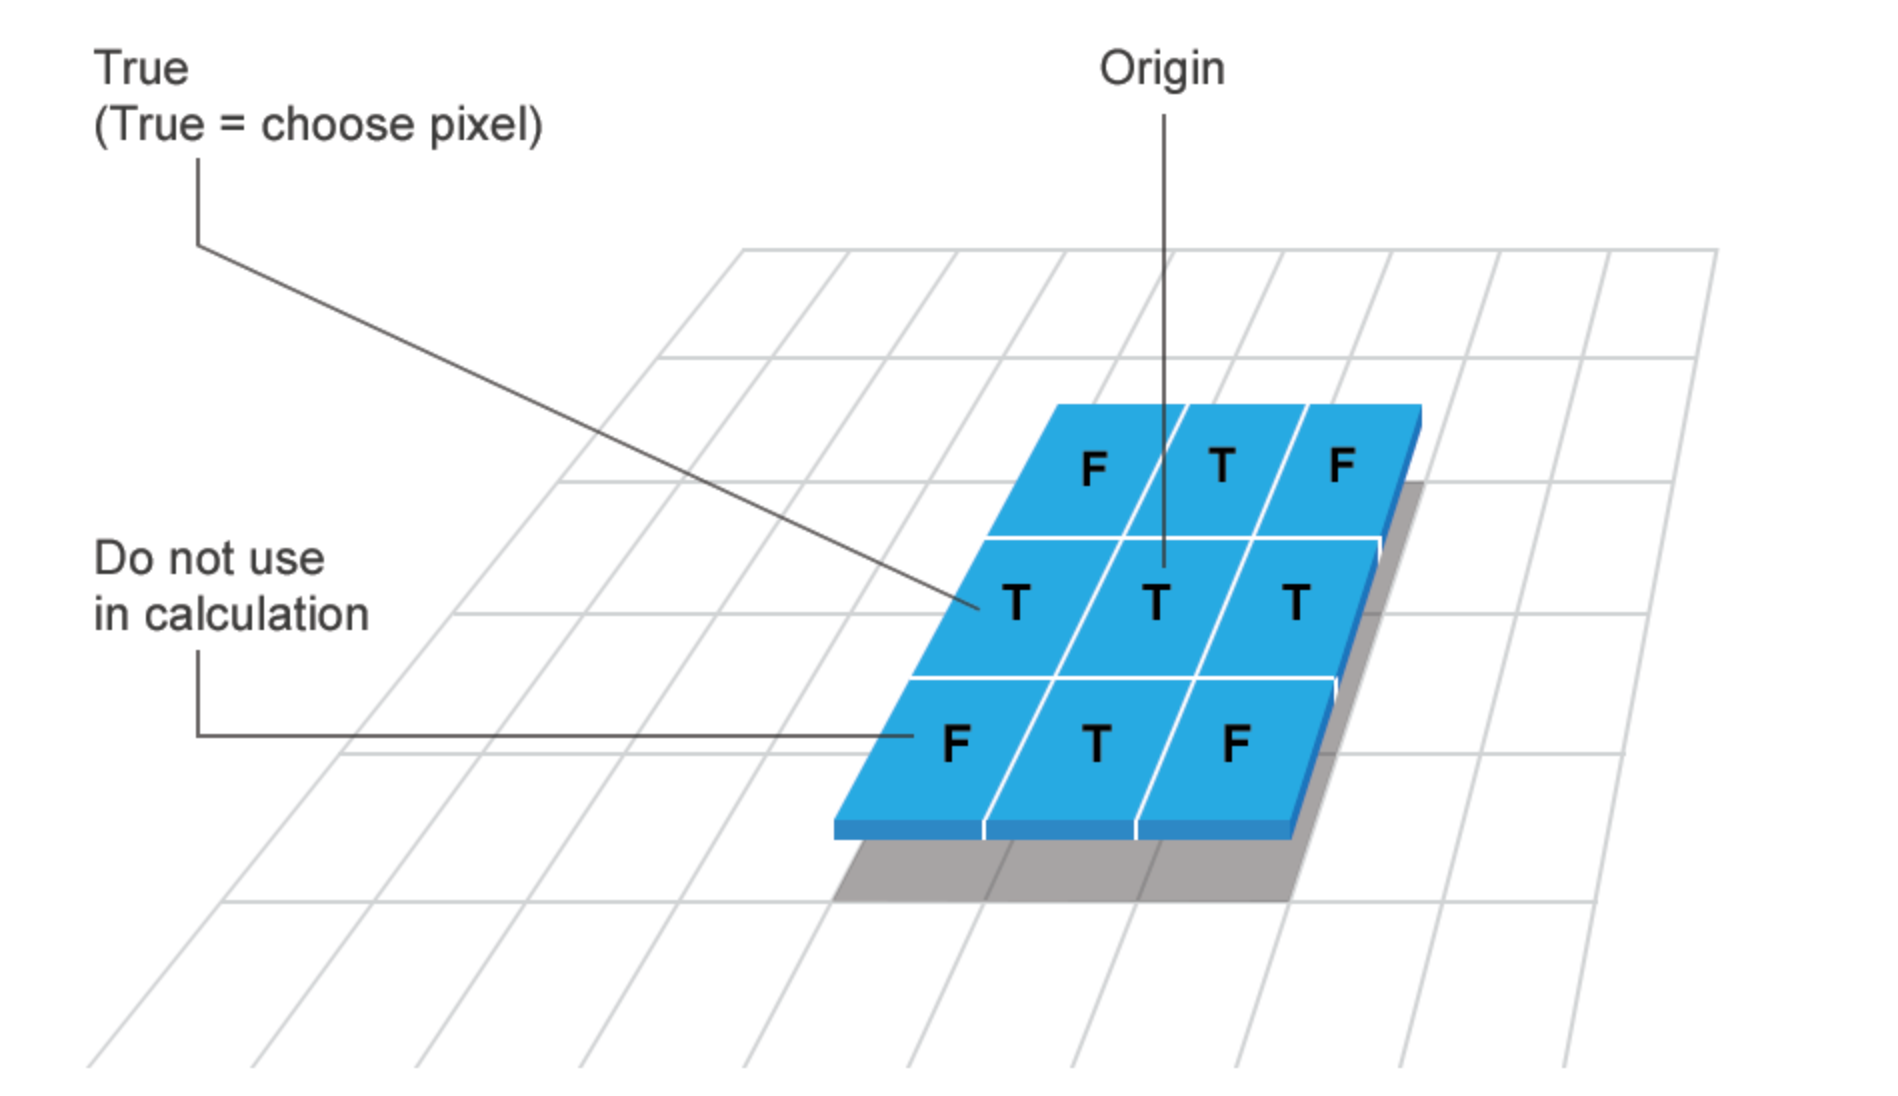
\includegraphics[width=0.5\linewidth]{bilder/structuring-element.png}
		\caption{Structuring Element}\label{fig:structuring-element}
	\end{center}
\end{figure}

Rolling ball algorithms
\begin{figure}[htb]
	\begin{center}
		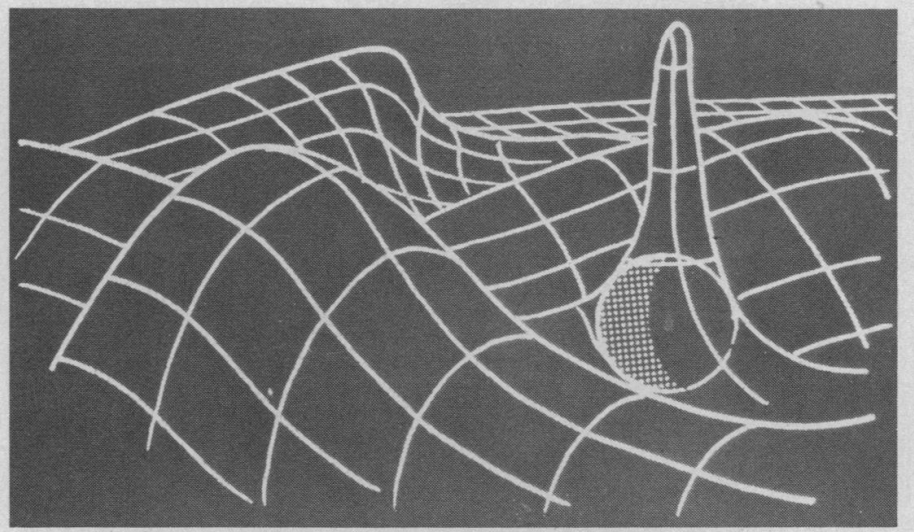
\includegraphics[width=0.5\linewidth]{bilder/rolling-ball.png}
		\caption{Rolling Ball}\label{fig:rolling-ball}
	\end{center}
\end{figure}

Rolling ball still leaves some noise


\begin{figure}
	\centering
	\begin{subfigure}[b]{0.22\textwidth}
		\centering
		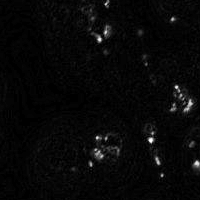
\includegraphics[width=\textwidth]{bilder/preprocessing/crop_golgi_not_full_processed.png}
		\caption{}
		\label{subfig:vanilla}
	\end{subfigure}
	\hfill
	\begin{subfigure}[b]{0.22\textwidth}
		\centering
		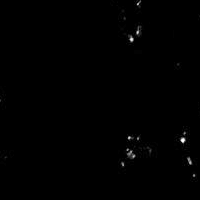
\includegraphics[width=\textwidth]{bilder/preprocessing/crop_golgi_full_processed.png}
		\caption{}
		\label{subfig:clipping}
	\end{subfigure}
	\hfill
	\begin{subfigure}[b]{0.22\textwidth}
		\centering
		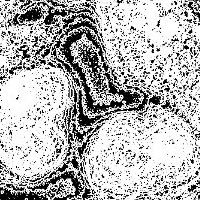
\includegraphics[width=\textwidth]{bilder/preprocessing/crop_golgi_not_full_processed_mask.png}
		\caption{}
		\label{subfig:vanilla-mask}
	\end{subfigure}
	\hfill
	\begin{subfigure}[b]{0.22\textwidth}
		\centering
		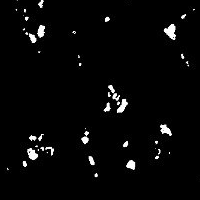
\includegraphics[width=\textwidth]{bilder/preprocessing/crop_golgi_full_processed_mask.png}
		\caption{}
		\label{subfig:clipping-mask}
	\end{subfigure}
	   \caption{(a) Vanilla pre-processing with automatic background removal algorithm only; (b) Additional clipping of lower intensities after vanilla pre-processing; (c) masked or subfigure (a); (d) mask of subfigure (b)}
	   \label{fig:pre-processing-golgi}
\end{figure}
